
\documentclass{jarticle}
\usepackage[truedimen,mag=850]{geometry}%フォントサイズを指定. 1000が10pt
\usepackage{geometry}
%\usepackage[dvipdfmx]{graphicx}
\usepackage{amssymb}%白抜き文字(mathbb)
\usepackage[dvipdfmx]{hyperref,graphicx}
\usepackage{pxrubrica}
\usepackage{bm}
\usepackage{amsmath}
\usepackage{ascmac}
\usepackage{comment}
\usepackage{url}
\usepackage{siunitx}
\usepackage{here}
\usepackage{listings}
\lstset{%
  language={Python},
  basicstyle={\small},%
  identifierstyle={\small},%
  commentstyle={\small\itshape\color[rgb]{0,0.5,0}},%
  keywordstyle={\small\bfseries\color[rgb]{0,0,1}},%
  ndkeywordstyle={\small},%
  stringstyle={\small\ttfamily\color[rgb]{1,0,1}},
  frame={tb},
  breaklines=true,
  columns=[l]{fullflexible},%
  numbers=left,%
  xrightmargin=0zw,%
  xleftmargin=3zw,%
  numberstyle={\scriptsize},%
  stepnumber=1,
  numbersep=1zw,%
  lineskip=-0.5ex%
}


\title{実験データ解析演習 最終レポート\\ 新潟県のお米の収量と天候の関連性について}
\author{2610180082 2年1組 No. 39  水野 響\ \\ 共同メンバー:藤波真尋, 山崎大知\\グループ番号:1}
\date{\today}
\begin{document}
\maketitle
\tableofcontents%目次を表示
\newpage


\section{研究背景}
一般的に, 農業はその土地の気候と密接に関係していることが知られており, その歴史は古い. 713年の諸国への風土記の編纂命令には「産物」の記載が含まれており, その頃には既に特産品に相当する概念が既にあったことがうかがえる. しかし現在, 気候変動や異常気象などで伝統的にその土地で育てられている農作物が不作となってしまうことや, 育てる農作物が変化している現状がある.

その中で古くから親しまれている日本人の主食, 米は日本各地で生産されており, 特に生産量1位である新潟県は古くからの日本で有数のお米の生産地である. そこで我々は新潟県とその気候を調べ, どのような要因が生産量に影響を与えているかを調べ, 天候から豊作不作を判定したいと考えた. また, その結果から他の土地に稲作の可能性を見出せると考える.

\hypertarget{header-n2003}{%
\section{目的}\label{header-n2003}}

\begin{enumerate}
\item 主成分分析で天候に大きく寄与する成分を見つける.
\item サポートベクターマシーンで新潟のお米の収量とその気候の関連性を調べる.
\end{enumerate}


\hypertarget{header-n2005}{%
\section{原理}\label{header-n2005}}


\hypertarget{header-n2009}{%
\subsection{サポートベクターマシン}\label{header-n2009}}

サポートベクターマシンでは,
自明に2群に線形分離可能である学習データを用いてその2群を最もよく分離する関数を考える.
個体あるいは対象を特徴づけるp個の変数
\(\bm{x} = (x_1, x_2, \cdots., x_p)^T\) に関して観測されたn個の学習データ$\bm{x}_1,\bm{x}_2,\cdots,\bm{x}_n$とする.
これらの学習データは2つの群$G_1, G_2$のどちらに属するものであるかが既に分かっているとする. 
ここで2群を分離する超平面
\[\bm{w}^T\bm{x} + b = 0\]
を考える. ここで, $\bm{w} = (w_1, w_2, \cdots, w_p)^T$とする.
線形分離可能な学習データに対しては分離超平面によってデータは$\bm{w}^T\bm{x}_i + b  > 0$または$\bm{w}^T\bm{x}_i + b < 0$のどちらかを満たす.
ここで($ \bm{w}^T\bm{x} + b > 0 : G_1,\ \bm{w}^T\bm{x} + b < 0 : G_2$)すなわち
\[\bm{x}_i \in G_1,\ \leftrightarrow  \bm{w}^T\bm{x} + b > 0,\ \ \ \bm{x}_i \in G_2,\ \leftrightarrow  \bm{w}^T\bm{x} + b < 0,\]


\begin{equation}
y = 
     \left\{
     \begin{aligned}
        1\ \ (\bm{x}_i\mbox{が} G_1 \mbox{に属するとき}) \\
        -1\ \ (\bm{x}_i\mbox{が} G_2 \mbox{に属するとき})\\
     \end{aligned}
     \right.
 \end{equation}
とすると 

全てのデータに対して
\[y_i(\bm{w}^T\bm{x}_i + b) > 0\]
が成り立つ.
 
 では, 線形分離可能な学習データに対してどのように超平面を構成すれば良いのだろうか.
 
このための基準として用いるのが距離である. 一般にp次元データ\(\bm{x} = (x_1, x_2, \cdots., x_p)^T\)から超平面$ \bm{w}^T\bm{x} + b = 0$上への距離は

 
 \[ d_i = \frac{|w_1x_{i1} + w_2x_{i2} + \cdots + w_px_{ip} + b|}{\sqrt{w_1^2 +\cdots+ w_p^2}} = \frac{|\bm{w}^T\bm{x}_i + b|}{||\bm{w}||}\]
 
 である.
 
 
\paragraph{マージン最大化}
 
 線形分離可能な場合は二軍を分離する1つの超平面$H$とそれを中間に挟む形で2つの超平面$ H_+, H_-$が存在する.
ここで, 両端の超平面には少なくとも1つのデータが存在し, その間にはデータは存在しないとする. サポートベクターマシーンでは, この$ H_+$と$ H_-$の中央にある$H$を最適な分離超平面と定義する.
 
 
 このため, 超平面$H_+$上のデータ$\bm{x}_+$あるいは$H_-$上のデータ$\bm{x}_-$から超平面$H$への距離
\[d = \frac{\bm{w}^T\bm{x}_+ + b}{||\bm{w}||} = \frac{-(\bm{w}^T\bm{x}_- + b)}{||\bm{w}||} \]

をマージンと呼び, 2群を最もうまく分類する問題を, このマージンを最大とする分離超平面を求める問題へと帰着させる. 
 
 つまり

\[\max_{\bm{w}, b} d\ \   s.t.\ \   \frac{y_i(\bm{w}^T\bm{x}_i + b)}{||\bm{w}||}\geq d \]

となる.
しかし, このマージン最大化問題の解を求めることは計算上難しいことから, 2次計画題とよばれる最適化問題ヘと式を変形する.

一般に超平面$  \bm{w}^T\bm{x} + b = 0$に任意の実数 $ \bm{r>0}$ をかけて, 係数のスケールを変えたとしても超平面は不変である.
 
 ここでマージン最大化の条件$\frac{|\bm{w}^T\bm{x}_i + b|}{||\bm{w}||}\geq d$に注目する.この両辺をマージンdで割ると, 
 \[y_i\left(\frac{\bm{w}^T\bm{x}_i}{d||\bm{w}||}+\frac{b}{d||\bm{w}||}\right)\geq 1\]
となる.
 
 
そこで, $r=1/d||\bm{w}||$とおいて係数のスケールを変えると, 上の式は
\[y_i(\bm{w}^{*\bm{T}}\bm{x_i}+b^*)\geq 1\]
というようになる.
ただし, 
\[\bm{w}^* = \frac{1}{d||\bm{w}||}\bm{w},\ \ \ \ \  b^* = \frac{1}{d||\bm{w}||}b\]
とおく.

 これは特に超平面$H_+,\ H_-$に対しては等号が成立する.
ゆえに, 等号が成立する超平面上のデータから分離超平面$H$上への距離, すなわちマージン$d^*$は
\[d^*=\frac{y_i(\bm{w}^{*T}\bm{x}_i+b^*)}{||\bm{w^*}||}=\frac{1}{||\bm{w}^*||}\]
となることがわかる.


以上のことから, スケール変換した分離超平面$\bm{w}^T\bm{x}_i+b^*=0$に対しては, 線形分離可能なすべての学習データは$y_i(\bm{w}^T\bm{x}_i+b^*)\geq 1$を満たしており, それゆえマージン最大化問題はこの不等式制約条件のもとでマージン$d^*=1/||\bm{w}^*||$を最大にする$\bm{w}^*$と$b^*$を求める問題に帰着する.

 また, マージン$d^*$の最大化は分母の重みベクトルのノルムの2乗$||\bm{w}||^{*2}$の最小化と同等であることから, マージン最大化問題は次のように定式化することができる.
ただし, $d^*,\ \bm{w}^*,\ b^*$はすべて, $d,\ \bm{w},\ b$と表記する.

\paragraph{主問題:マージン最大化問題}

\[\min_{\bm{w}}\frac{1}{2}||\bm{w}||^2,\ \ \ \ \ \ \mbox{制約条件}\ \ y_i(\bm{w}^{T}\bm{x}_i+b)\geq 1,\ \ \ \  i=1,2,\cdots,\ n\hspace{10mm}\cdots(1)\]

サポートベクターマーシンでは$(*)$を主問題としてラグランジュ関数を導入して双対問題と呼ばれる最適化問題に帰着させて解く.

まず制約条件の個数nに相当するラグランジュ乗数$\alpha_1,\ \alpha_2,\ \cdots,\ \alpha_n\ (\alpha_i \geq 0;\ i=1,2,\cdots, n)$を用いて, ラグランジュ関数
\[L(\bm{w}, b, \alpha_1, \alpha_2, \cdots, \alpha_n) = \frac{1}{2}||\bm{w}||^2 - \sum_{i=1}^n \alpha_i \left\{y_i (\bm{w}^T \bm{x}_i + b) - 1\right\} \ \ \ \ \ \ \cdots (*)\]を導入する.

次に, 重みベクトル$\bm{w}$と切片$b$でラグランジュ関数を偏微分した式を0とおくと

\[\frac{\partial L(\bm{w}, b, \alpha_1, \alpha_2, \cdots, \alpha_n)}{\partial \bm{w}} = \bm{w} - \sum_{i=1}^n \alpha_n y_i \bm{x}_i = \bm{0}\]

\[\frac{\partial L(\bm{w}, b, \alpha_1, \alpha_2, \cdots, \alpha_n)}{\partial b} = - \sum_{i=1}^n \alpha_n y_i = 0\]
となる. よって

\[\bm{w} = \sum_{i=1}^n \alpha_i y_i \bm{x}_i,\hspace{5mm} \sum_{i=1}^n \alpha_i y_i = 0\ \ \cdots(2)\]
 を得る.
 
\[L_D (\alpha_1, \alpha_2, \cdots, \alpha_n) =  \sum_{i=1}^n \alpha_i  - \frac{1}{2} \sum_{i=1}^n  \sum_{j=1}^n \alpha_i \alpha_j y_i y_j \bm{x}_i^T\bm{x}_j\]
 が求まる.
 
このようにして主問題$(1)$をラグランジュ関数に関する最適化問題へと帰着させる.
 
 \[\max_{\alpha_1, \alpha_2, \cdots, \alpha_n} L_D (\alpha_1, \alpha_2, \cdots, \alpha_n)  = \max_{\alpha_1, \alpha_2, \cdots, \alpha_n} \left\{ \sum_{i=1}^n \alpha_i  - \frac{1}{2} \sum_{i=1}^n  \sum_{j=1}^n \alpha_i \alpha_j y_i y_j \bm{x}_i^T\bm{x}_j \right\},\]
 \[\mbox{制約条件:}\ \ \alpha_i \geq 0 \ \ (i=1,2,\cdots,n),\ \ \sum_{i=1}^n \alpha_i y_i = 0\]
 
この双対問題の解を$\hat{\alpha_1}, \hat{\alpha_2}, \cdots, \hat{\alpha_n}$とすると, 式(2)の重みベクトル$\bm{w}$に含まれるラグランジュ乗数を双対問題の解で置き換えることにより最適解
\[\hat{\bm{w}} = \sum_{i=1}^n \hat{\alpha}_i y_i \bm{x}_i\]
を得る. また切片$b$については
\[H_+ : \hat{\bm{w}}^T \bm{x}_+ + b = 1,\hspace{10mm} H_- : \hat{\bm{w}}^T\bm{x}_- + b = -1\]
 が成り立つことを用いると, 
 \[\hat{b} = -\frac{1}{2}(\bm{w}^T \bm{x}_+ + \bm{w}^T \bm{x}_-)\]
 が求まる.
 以上より線形分離可能である学習データに対してマージンが最大となる2群を分離する超平面は
 \[\hat{\bm{w}}^T \bm{x} + \hat{b} = \sum_{i=1}^n \hat{\alpha}_i y_i \bm{x}_i^T \bm{x} + \hat{b} = 0\]
である. 従って最適な分離超平面を判別関数とする2群$G_1,\ G_2$の判別法は
 
\begin{equation*}
\hat{\bm{w}}^T \bm{x} + \hat{b} = \sum_{i=1}^n \hat{\alpha}_i y_i \bm{x}_i^T \bm{x} + \hat{b} 
     \left\{
     \begin{aligned}
       \geq 0 \Longrightarrow\ \ G_1\\
       < 0 \Longrightarrow\ \ G_2\\
     \end{aligned}
     \right.\ \ \ \ \ \ \ \cdots(3)
 \end{equation*}

で与えられる. サポートベクターマシンは実質的に判別関数を構築するデータは最適な超平面を挟む2つの超平面$H_-,H_+$上のデータ, すなわち
\[y_i (\hat{\bm{w}}^T \bm{x}_i + \hat{b}) = 1\]
を満たすデータのみである. それらのデータはサポートベクターと呼ばれ, サポートベクターによって構成される識別機をサポートベクターマシンという. 従って, サポートベクターの添字集合をSとすると, (3)は
\begin{equation*}
\hat{\bm{w}}^T \bm{x} + \hat{b} = \sum_{i\in S} \hat{\alpha}_i y_i \bm{x}_i^T \bm{x} + \hat{b} 
     \left\{
     \begin{aligned}
       \geq 0 \Longrightarrow\ \ G_1\\
       < 0 \Longrightarrow\ \ G_2\\
     \end{aligned}
     \right.\ \ \ \ \ \ \ \cdots(4)
 \end{equation*}

と表せる.

サポートベクターマシンの大きな特徴は, 次のKarush-Kuhn-Tucker条件から導かれることが知られている.


\paragraph{Karush-Kuhn-Tucker条件}

p次元実数値関数を$f(w_1, \cdots w_p) = f(\bm{w})$とする. この目的関数を最小とする解を, n個の不等式制約条件$g_i(\bm{w}) \leq 0,\ i=1,2,\cdots,n$のもとで求めるとする.
すなわち, 

\[\min_{\bm{w}} f(\bm{w}),\ \ \ \ \ \ \mbox{制約条件}\ \ g_i(\bm{w})\leq 0,\ \ \ \  i=1,2,\cdots,\ n\hspace{10mm}\cdots(5)\]

次にラグランジュ乗数$\bm{\alpha} = (\alpha_1,\cdots \alpha_n)^T$を導入したラグランジュ関数を

\[L(\bm{w}, \bm{\alpha}) = f(\bm{w}) + \sum_{i=1}^n \alpha_i g_i (\bm{w}) \ \ \cdots (6)\]

とする. このとき, 不等式制約条件下での最適化問題は次の4つの条件を満足する重みベクトル$\bm{w}$とラグランジュ乗数$\bm{\alpha}$を求める問題に帰着される.

\[(1)\ \ \frac{\partial L(\bm{w}, \bm{\alpha})}{\partial w_i} = 0\ \ \ \hspace{16mm} \ \ \ i=1,2,\cdots, p\]
\[(2)\ \ \frac{\partial L(\bm{w}, \bm{\alpha})}{\partial \alpha_i} = g_i(\bm{w}) \leq 0\hspace{10mm} i=1,2,\cdots, n\]
\[(3)\ \ \ \alpha_i \geq 0\ \ \hspace{30mm}\ i=1,2,\cdots,n\]
\[(4)\ \ \ \ \alpha_i g_i(\bm{w}) = 0\ \ \hspace{10mm} \ \ \ \ \ \ \ \ \ \ i=1,2,\cdots,n\]

\paragraph{サポートベクター}

マージンを最大とするという意味で最適な分離超平面を求めるために用いた式$(*)$のラグランジュ関数は, 目的関数$f(\bm{w})$と制約条件式$g_i(\bm{w})$をそれぞれ
\[f(\bm{w} = \frac{1}{2}||\b{w}||^2,\ \ g_i(\bm{w}) = -\left\{ y_i (\bm{w}^T\bm{x}_i + b) - 1\right\}\ \ \ \ i=1,2,\cdots, n\]
とおいたものである.
このとき, Karush-Kuhn-Tucker条件の一つである(4)に対して

\[\alpha_i \{y_i (\bm{w}^T \bm{x} + b) - 1\} = 0,\ \ \ \ \ \ i=1,2,\cdots,n\]

が成り立っていることを示している. データがサポートベクターでない場合は$y_i(\bm{w}^T \bm{x} + b) >1$となり, 上式より$\alpha_i = 0$となる. 一方サポートベクターに対しては$y_i(\bm{w}^T \bm{x} + b) = 1$が成り立ち, $\alpha_i > 0$が成り立つ. 従って式(4)の判別関数を構成するデータは, $\alpha_i > 0$に対応するサポートベクターのみであることが示される.

\hypertarget{header-n2013}{%
\section{データ}\label{header-n2013}}
使用したデータの種類と出典は表\ref{data}の通りである.

\begin{table}[H]
\caption{使用したデータの種類と出典}
\begin{tabular}{|c|c|c|c|} \hline
&データの種類&出典\\ \hline
米の収量&10aあたりの収量 (t)&eStat\\ \hline
天気&日照時間, 気温, 湿度, 降水量, 風速, 雲量&気象庁\\ \hline
\end{tabular}
\centering
\label{data}
\end{table}


\hypertarget{header-n2026}{%
\section{操作}\label{header-n2026}}

\begin{enumerate}
\def\labelenumi{\arabic{enumi}.}
\item
  6次元の気候データを主成分分析により2次元に圧縮した.
\item
  収量を480 (t)以上の年を豊作とし, ラベルを豊作の年を1,
  不作の年を0としてラベル付けをした.
\item
  主成分分析した2次元データと固有ベクトルを月ごとにプロットした.
\item
  第一主成分と第二主成分の配列を用意した.
\item
  主成分をtrainデータとtestデータを7:3の割合で分割した.
\item
  サポートベクターマシーンを学習させた.
\item
  サポートベクターマシーンの正答率を求めた.
\item
  横軸を第一主成分, 縦軸を第二主成分としてデータをプロットし,
  サポートベクターマシーンの分類結果を可視化した.
\item
  以上を12ヶ月分同様に行った.
\item
  result配列を用意し,
  月ごとの第一主成分と第二主成分とサポートベクターマシーンの正答率を格納した.
\end{enumerate}

\hypertarget{header-n2048}{%
\section{結果}\label{header-n2048}}

操作3による散布図が図\ref{pca}である. 操作8による散布図が図\ref{svm}である.
%小さくて見えないかもしれないが, rainfallは降水量, sunlightは日照時間を示している.(他も書く?)

月ごとの第一主成分と第二主成分とサポートベクターマシーンの正答率が表\ref{score}である.
オレンジ色の方が豊作で, 青色の部分が不作を表している.

\begin{figure}[H]
\centering
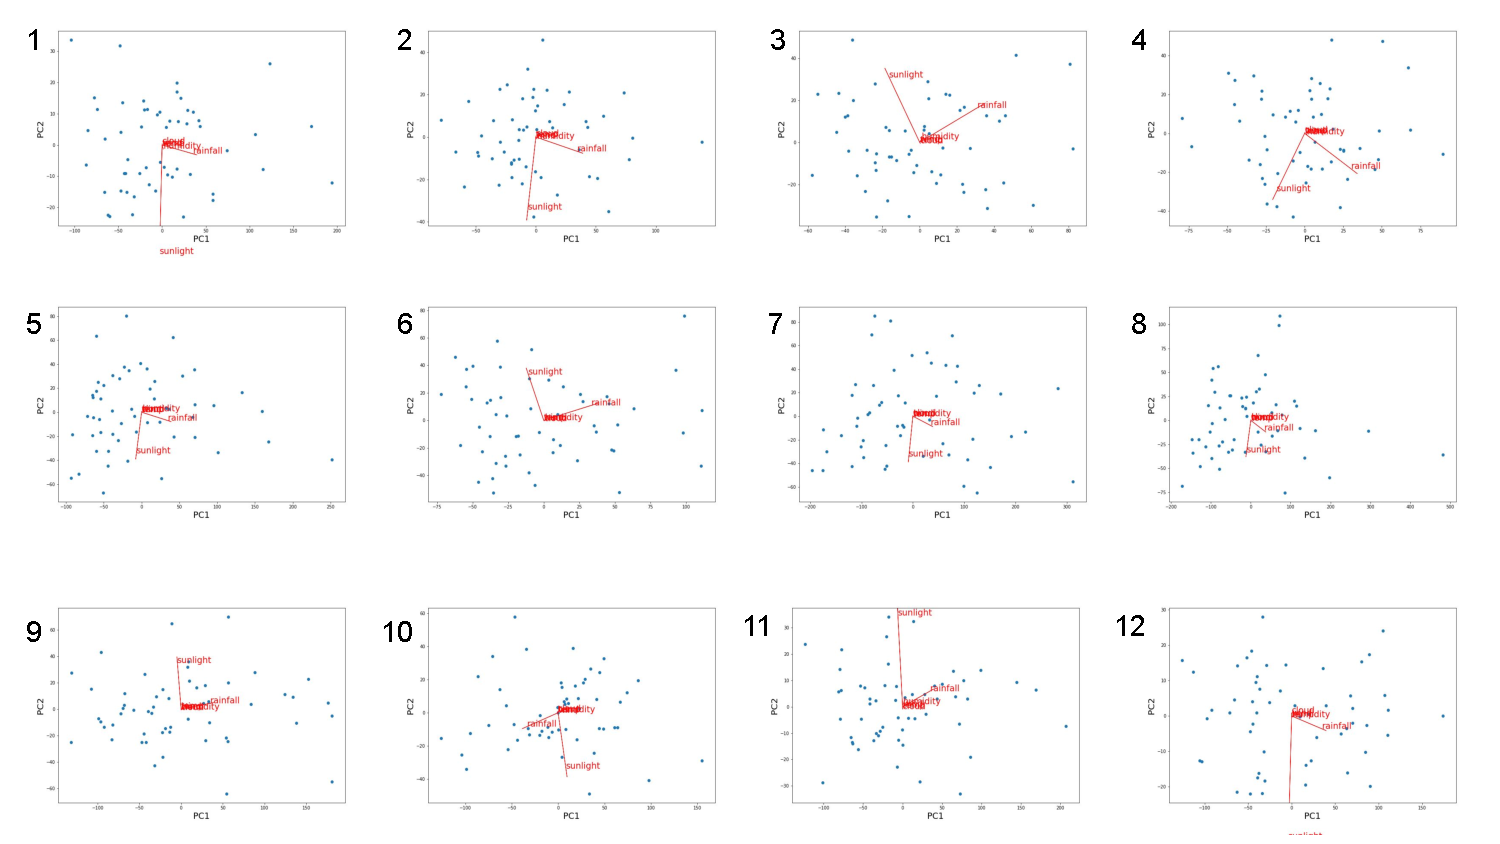
\includegraphics[keepaspectratio, scale=0.75]
{pca_plot.pdf}
\caption{主成分分析による分析結果}
\label{pca}
\end{figure}



\begin{figure}[H]
\centering
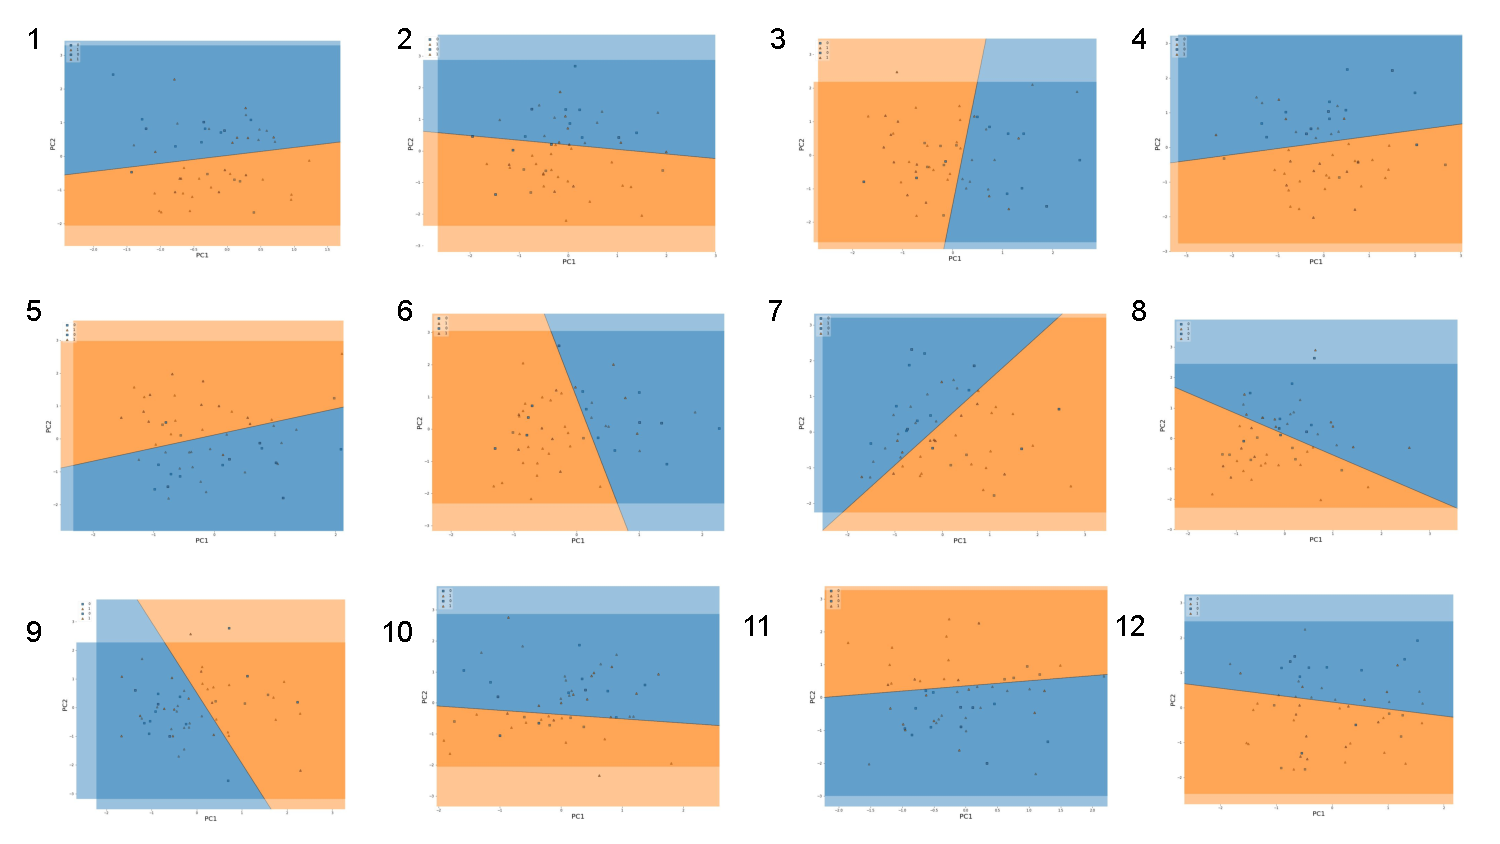
\includegraphics[keepaspectratio, scale=0.75]
{svm_plot.pdf}
\caption{サポートベクターマシンによる分析結果}
\label{svm}
\end{figure}

%\begin{lstlisting}[caption=score, label=score]
%           PC1       PC2  SVM_score
% month                               
% 1       0.948290    0.049088   0.529412
% 2       0.841302    0.151448   0.352941
% 3       0.726571    0.266117   0.588235
% 4       0.707992    0.285218   0.705882
% 5       0.718615    0.278711   0.882353
% 6       0.835200    0.163343   0.529412
% 7       0.907491    0.091873   0.588235
% 8       0.902660    0.096692   0.352941
% 9       0.906668    0.092054   0.3520961
% 10      0.867753    0.129710   0.235294
% 11      0.953945    0.043966   0.470588
% 12      0.965803    0.031950   0.5882
%\end{lstlisting}
\begin{table}[H]
\caption{月ごとの固有ベクトルとSVM正答率}
\begin{tabular}{|c|c|c|c|} \hline
month&PC1&PC2 &SVM\_score\\ \hline
 1&0.948290&0.049088&0.529412\\ \hline
 2&0.841302&0.151448&0.352941\\ \hline
 3&0.726571&0.266117&0.588235\\ \hline
 4&0.707992 &0.285218&0.705882\\ \hline
 5&0.718615&0.278711&0.882353\\ \hline
 6&0.835200&0.163343&0.529412\\ \hline
 7&0.907491&0.091873&0.588235\\ \hline
 8&0.902660&0.096692&0.352941\\ \hline
 9&0.906668&0.092054&0.352096\\ \hline
 10&0.867753&0.129710&0.235294\\ \hline
 11&0.953945&0.043966&0.470588\\ \hline
 12&0.965803&0.031950&0.588200\\ \hline
\end{tabular}
\centering
\label{score}
\end{table}


\hypertarget{header-n2056}{%
\section{考察}\label{header-n2056}}
以下, 第一主成分をPC!, 第二主成分をPC2, サポートベクターマシンをSVMと略す.
第二主成分の寄与率が高い月はSVMの正答率が高い. 特に5月はSVMの正答率が高い. それら以外はあてになる分析結果とはいえない. ここでは表\ref{score}からSVMの正答率が$0.7$を超えている4月と5月について考える. 
4月は図\ref{svm}からPC1の影響はほぼ関係がなく, PC2の影響のみを考える. 図\ref{pca}のPCAの固有ベクトルと図\ref{svm}のSVMの結果から, 日照時間が長ければ豊作になり, 降水量は関係がない.

5月は4月同様, 降水量は関係がなく, 日照時間は短い方が豊作になる.

ところで, 4月は稲作では種籾を用意して発芽させてタネを育苗箱に蒔き, その後ハウス内で苗を育てる時期に相当する. すなわち4月の天候, 特に降水量と日照時間は稲作の様々な要因のうち, 田んぼの土のみに影響を与えると考えられる. 一般的に土に日光を当てる行為は, 日光消毒として知られている. そのため, 稲作においては4月における土の日光消毒が重要な役割を担っていると考えられる.

また. 5月は田おこしをし, しろかき(水を引き入れてトラクターでよく混ぜる)を行った後, 田植えを行う時期である. 植えたばかりの稲は弱いので水を深めのまま管理する深水管理を行うことが知られていることから, 日照時間が短い方が良いということはこれに係る水の蒸発が稲作に良い影響を及ぼさないということが読み取れる.

すなわち以上をまとめると, 稲作は4月の田んぼの日光消毒と, 5月の深水管理が最も需要な豊作の因子であることが考えられる.

%だからとりあえず4月5月のみを考える
%4月はPC2の影響のみを考えればよくて, PC1は関係ない. つまり, PCAの固有ベクトルとSVMの結果から, 日照時間が長ければ豊作になり, 降水量は関係ない
%5月は4月同様に, 降水量は関係なくて, 日照時間は短い方が豊作になる.
%4,5月ってどういう時期だ??稲植えてる?
%4月は種籾を用意して発芽させてタネを育苗箱に蒔く. その後, ハウス内で苗を育てる. 
%土に日光を当てておく?と?どんな影響があんの?
%日光消毒.
%5月は田おこし. しろかき(水を引き入れてトラクターでよく混ぜる). そして田植え.
%水を引くわけだから, 晴れちゃうと干からびちゃうのかな?

\section{次への課題}
\begin{itemize}
\item 4月, 5月以外のSVMによる分析が使い物にならなかった. 次元拡張をすれば分離できたかもしれない. 
\item 他地域の気候を調べ, 稲作に最適な地域を洗い出したかった.
\item 他の班が行っていたように, 前処理の段階で箱ひげ図などで可視化し, ある程度の仮説を用意すべきだった.
\item 12ヶ月分の分析を行うと, 結果が非常に見づらいものになってしまった. 季節ごと(3ヶ月)で区切るべきだった.
\end{itemize}

%ある程度仮説を立てるべきだった.
\begin{thebibliography}{9}
  %\bibitem{1} 並木雅俊 「大学生のための物理入門」P.95, 98 (2010).
%  \bibitem{1}\href{https://re-imagej.blogspot.com/2015/09/252.html}{Re - ImageJで学ぶ : 第25回 2値化の応用 医用画像の特徴量解析 フラクタル解析で学ぶ}\url{https://re-imagej.blogspot.com/2015/09/252.html}
  \bibitem{1} 小西貞則「多変量解析入門——線形から非線形へ」p.193$\sim$203
  \bibitem{2}\href{  https://www.kankou-shimane.com/shinwa/kiso/fudoki/index.html}{出雲国風土記}\url{  https://www.kankou-shimane.com/shinwa/kiso/fudoki/index.html}
 \bibitem{3}\href{ http://www.jmmp.jp/difference.html }{特産品と名産品の違い}\url{http://www.jmmp.jp/difference.html}
 \bibitem{4}\href{ http://ytnk.jp/tanadakai/kometukuri.html}{お米ができるまで}\url{http://ytnk.jp/tanadakai/kometukuri.html}
 \bibitem{5}\href{https://www.nihonbunka.or.jp/tanbo }{田んぼ学校}\url{https://www.nihonbunka.or.jp/tanbo}

\end{thebibliography}
\end{document}
